\documentclass[11pt]{article}
\usepackage[margin=2.5cm]{geometry}
\usepackage{amsmath,amssymb,booktabs,graphicx}
\title{Uniaxial anisotropy on tetrahedral spin bodies:\\
axis selection and exact effective $O(2)$ models}
\author{Note for the Polyhedron\_Spin\_Group follow-up}
\date{3 November 2026}
\begin{document}
\maketitle

\section{Setup}
We add a single-spin anisotropy to the $n=4$ model of the main paper,
\begin{equation}
V=\sum_a\sum_{i=1}^{4}\big[a_2P_2(\hat z\cdot\mathbf S_{a,i})+a_4P_4(\hat z\cdot\mathbf S_{a,i})\big],
\end{equation}
with $a_2=2D/3$ for $D(S^z)^2$ and $a_4=8B/35$ for $B(S^z)^4$ (the $P_2$ part of
$B(S^z)^4$ adds to $a_2$). $V$ is a sum of single-body terms, so the uniform-state
theorem still holds and the problem reduces to one body with pair potential
$\Phi(x)=\sum_l\kappa_lP_l(x)$, $\kappa_l=f_l-zg_l$. The deformation stiffnesses
$\lambda_E,\lambda_{T_2}$ of Eq.~(9) of the main paper therefore already contain the
inter-body couplings. The symmetry is reduced from $O(3)$ to $D_\infty\times\mathbb Z_2^T$.

\section{First order: the two-design removes $a_2$}
Because the tetrahedron is a spherical 2-design, $\sum_i(\hat z\cdot\mathbf S_i)^2=4/3$
for every orientation, so the $a_2$ term has no first-order effect. The $a_4$ term
is the $l=4$ cubic harmonic. With $K\equiv\sum_\alpha n_\alpha^4$, where $\hat n$ is
$\hat z$ in the cube frame of the body ($K=1$ for an $S_4$ axis, $K=1/3$ for a $C_3$
axis),
\begin{equation}
E^{(1)}=a_4\Big(\frac73-\frac{35}{9}K\Big).
\end{equation}

\section{Second order: selection through deformation}
At first order the energy does not depend on orientation, so there is no torque.
The force acts only on the $E$ and $T_2$ deformation modes. The force on spin $i$ is
$3a_2(\hat z\cdot\mathbf S_i)\,[\hat z-(\hat z\cdot\mathbf S_i)\mathbf S_i]$. At the
symmetric orientations it lies entirely in one representation:
\begin{align}
S_4\parallel\hat z&:\quad |f_E|^2=4\cdot9\cdot\tfrac13\cdot\tfrac23\,a_2^2=8a_2^2,
\quad f_{T_2}=0,\\
C_3\parallel\hat z&:\quad |f_{T_2}|^2=3\cdot9\cdot\tfrac19\cdot\tfrac89\,a_2^2=\tfrac83a_2^2,
\quad f_E=0 .
\end{align}
The $5$-dimensional $l=2$ force splits as $E\oplus T_2$ under $T_d$, with weights
$(3K-1)/2$ and $3(1-K)/2$. The result is again linear in $K$:
\begin{equation}
E^{(2)}=-\tfrac12\Big[\frac{|f_E|^2}{\lambda_E}+\frac{|f_{T_2}|^2}{\lambda_{T_2}}\Big]
=-2a_2^2\Big(\frac{3}{\lambda_E}-\frac{1}{\lambda_{T_2}}\Big)K+\text{const}.
\end{equation}
In terms of derivatives of $\Phi$ at the tetrahedral angle, Eq.~(9) of the main paper reads
\begin{equation}
\lambda_E=\tfrac83\,\Phi''(-\tfrac13),\qquad
\lambda_{T_2}=\tfrac89\big[3\Phi'(-\tfrac13)+2\Phi''(-\tfrac13)\big].
\end{equation}

\paragraph{Result.}
\begin{equation}
\boxed{E_{\rm eff}(\hat n)=-\Gamma\sum_\alpha n_\alpha^4,\qquad
\Gamma=\frac{35}{9}a_4+2a_2^2\Big(\frac{3}{\lambda_E}-\frac{1}{\lambda_{T_2}}\Big)}
\end{equation}
$\Gamma>0$ selects an $S_4$ axis along $\hat z$, $\Gamma<0$ a $C_3$ axis. The second-order
term does not depend on the sign of $D$ (easy axis or easy plane).
Direct numerical minimization for five random $\kappa$ sets and three anisotropy
combinations agrees with this formula to better than 1\%.

\section{Selection criterion: $\kappa_2$ cancels}
\begin{equation}
3\lambda_{T_2}-\lambda_E=\frac{8}{27}\,(27\kappa_1-63\kappa_3+35\kappa_4)
=\frac{8}{27}\,(27J+9zG-8zH_4).
\end{equation}
\begin{itemize}
\item In the whole T phase of the $(zG,zH_4)$ plane at $K=0.5$ this is positive, so the
deformation channel always selects $S_4\parallel\hat z$.
\item $C_3\parallel\hat z$ requires either $a_4<-\frac{18}{35}a_2^2(3/\lambda_E-1/\lambda_{T_2})$
(quartic single-ion anisotropy wins) or, at large $K$, the window $8zH_4>27J+9zG$.
\item As $K\to0$, $\lambda_E\propto K\to0$: perturbation theory fails and $S_4$ selection
becomes strong.
\end{itemize}

\section{Exact effective models of the selected phases}
For a rigid tetrahedron only the $l=3$ and $l=4$ channels couple bodies ($l=1,2$ vanish for a
2-design), with $g_3=\frac25G$, $g_4=\frac{8}{35}H_4$. The bond energy is
$-g_l\frac{4\pi}{2l+1}\,\mathrm{Re}\,\mathbf q^{(l)}_a\cdot\mathbf q^{(l)*}_b$.
The multipole weights (checked numerically) are:
\begin{center}
\begin{tabular}{lcc}
\toprule
axis & $l=3$ & $l=4$\\
\midrule
$S_4$ & $m=\pm2$: $80/9$ & $m=0$: $196/81$; $m=\pm4$: $140/81$\\
$C_3$ & $m=0$: $400/81$; $m=\pm3$: $320/81$ & $m=0$: $784/729$; $m=\pm3$: $2240/729$\\
\bottomrule
\end{tabular}
\end{center}

\subsection*{$S_4\parallel\hat z$: generalized XY model ($q=2$)}
With $\theta=2\alpha$ ($\alpha$ the in-plane body angle),
\begin{equation}
H=-\sum_{\langle ab\rangle}\Big[\frac{32}{9}G\cos(\theta_a-\theta_b)+\frac{32}{81}H_4\cos2(\theta_a-\theta_b)\Big].
\end{equation}
Time reversal acts as $\theta\to\theta+\pi$. The polar phase is octupolar order; the
half-vortex ``nematic'' phase is the time-reversal-even hexadecapolar phase, the 2D version
of the $T_d\subset O_h$ (cubatic) vestigial phase. The mixing ratio is fixed microscopically,
$\Delta/(1-\Delta)=9G/H_4$, so the vestigial phase needs $H_4/G$ of order 20.

\subsection*{$C_3\parallel\hat z$: coupled Ising--XY model}
Let $\sigma=\pm1$ label up/down tetrahedra (related by time reversal) and
$\varphi=3\alpha+\pi(1-\sigma)/2$. Then
\begin{equation}
H=-\sum_{\langle ab\rangle}\Big[\frac{160}{81}G\,\sigma_a\sigma_b
+\Big(\frac{128}{81}G+\frac{512}{729}H_4\,\sigma_a\sigma_b\Big)\cos(\varphi_a-\varphi_b)\Big].
\end{equation}
\begin{itemize}
\item For $H_4=0$ the Ising and XY variables decouple exactly: the octupolar channel alone
cannot mix $\sigma\sigma'$ with $\cos(\varphi-\varphi')$. Square-lattice estimates:
$T_{\rm Ising}\approx1.12\,zG$ above $T_{\rm KT}\approx0.35\,zG$.
\item $H_4$ switches on the coupling, $J_4/J_2=\frac49\,zH_4/zG$. At $J_4=J_2$ the model has the
Granato--Kosterlitz--Lee--Nightingale form studied for the fully frustrated XY model.
The coupling is thus tuned continuously from zero by a single microscopic ratio.
\item A $2\pi$ vortex of $\varphi$ is a $2\pi/3$ vortex of the body; an Ising domain wall twists
$\alpha$ by $\pi/3$.
\end{itemize}

\paragraph{Small $\Gamma$.} In 2D the $SO(3)/T$ correlation length grows as $\exp(c/T)$, so the
effective anisotropy $\xi^2\Gamma$ is relevant. Transitions exist for any $\Gamma\neq0$, with
transition temperatures reduced logarithmically for small $\Gamma$.

\section{Two exactly decoupled limits of the $C_3$ model}
With $\psi=3\alpha$ the same Hamiltonian reads
\begin{equation}
H=-\sum_{\langle ab\rangle}\big[J_1\sigma_a\sigma_b+(J_2\sigma_a\sigma_b+J_4)\cos(\psi_a-\psi_b)\big],
\end{equation}
$J_1=\frac{160}{81}G$, $J_2=\frac{128}{81}G$, $J_4=\frac{512}{729}H_4$, $r\equiv J_4/J_2=\frac49 zH_4/zG$.
\begin{itemize}
\item $J_4=0$ ($H_4=0$): $\sigma$ and $\varphi=\psi+\pi(1-\sigma)/2$ decouple. The octupole sign
(TR odd) orders first, at $T_I=2.269J_1$; the full octupole $\varphi$ follows at
$T_{\rm KT}=0.893J_2$.
\item $J_2\to0$ ($G\to0$): $\sigma$ and $\psi$ decouple. The TR-even hexadecapole $\psi$
($l=4$, $m=\pm3$) orders by itself.
\end{itemize}
The two limits have opposite order of transitions, so the Ising and KT lines must cross at
some $r_\times$. Leading-order estimates of both lines:
\begin{equation}
T_{\rm KT}\simeq0.893\,(J_2+J_4\langle\sigma\sigma'\rangle)\xrightarrow{\ \sigma\ \text{ordered}\ }0.893(1+r)J_2,
\end{equation}
\begin{equation}
T_I=2.269\Big[J_1+\frac{T_I}{2}\ln\frac{I_0\big((J_2+J_4)/T_I\big)}{I_0\big(|J_2-J_4|/T_I\big)}\Big]
\quad(\text{tree integration of }\varphi),
\end{equation}
and $T_I\le2.269(J_1+J_2)\approx8.07\,G$ once $\psi$ is ordered.

\section{Monte Carlo of the $C_3$ effective model}
Square lattice, $L=16,32,48$, Metropolis plus Wolff clusters in both sectors ($\sigma$ at fixed
$\varphi$ with bond $J_1+J_4\cos\Delta\varphi$; embedded $\varphi$ at fixed $\sigma$ with bond
$J_2+J_4\sigma\sigma'$; both valid for either sign), annealed downward in $T$.
Ising $T_I$ from Binder crossings and the collapse of $|m_\sigma|$; KT from
$\Upsilon_\varphi=2T/\pi$ at $L=48$ (twisting $\varphi$ or $\psi$ gives the same $\Upsilon$).
\begin{center}
\begin{tabular}{ccc}
\toprule
$r$ & $T_I/G$ & $T_{\rm KT}(L=48)/G$\\
\midrule
0 & 4.50 & 1.46\\
1 & 5.13 & 2.90\\
2 & 5.76 & 4.31\\
3 & 6.45(12) & 5.63\\
3.5 & 6.82 & 6.24\\
4 & 7.11 & 6.82\\
4.5 & 7.00(10) & 7.32\\
5 & 7.35 & 7.89\\
\bottomrule
\end{tabular}
\end{center}
\begin{itemize}
\item $r=0$ reproduces the decoupled values ($2.269J_1=4.48$; $0.893J_2=1.41$ with the usual
$L=48$ upward shift).
\item For $r\le2$ the KT line follows $0.893(1+r)J_2$ and $T_I$ follows the tree estimate.
\item The lines cross at $r_\times\approx4.2\pm0.2$, i.e.\ $zH_4/zG\approx9.5$. Above it the order
is reversed: an intermediate phase with quasi-long-range $\psi$ order and disordered $\sigma$
appears. This is the TR-even hexadecapolar (vestigial) phase of the tilted tetrahedra; its
elementary vortex is a $2\pi/3$ rotation of the body.
\item Near $r_\times$ the Binder cumulant occasionally becomes negative at $L=48$, which may signal a
weakly first-order merged transition; the present sampling (no parallel tempering) does not
decide this.
\end{itemize}

\begin{center}
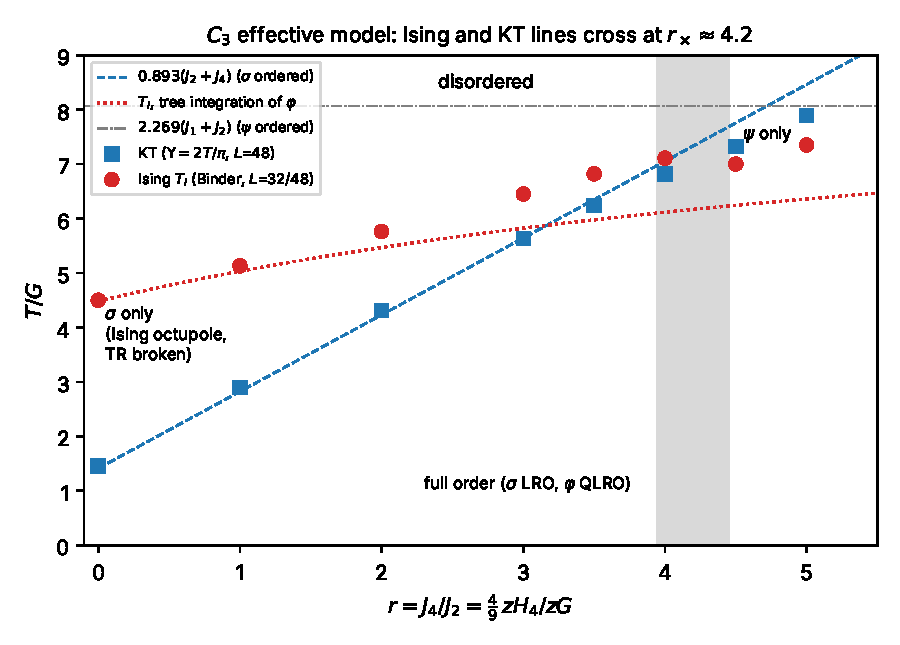
\includegraphics[width=0.75\textwidth]{phase_diagram_C3.pdf}
\end{center}

\section{Dependency chain and next step}
\[
\kappa_l\ \to\ (\lambda_E,\lambda_{T_2})\ \to\ \Gamma\ \to\ \text{selected axis}\ \to\
\text{effective 2D model with couplings fixed by }(G,H_4)\ \to\ \text{phase sequence}.
\]
Open: nature of the transitions near $r_\times$ (parallel tempering, energy histograms,
$L\ge64$) and whether the physical $(K,zG,zH_4)$ window for $C_3$ selection reaches $r_\times$.

\end{document}
